\documentclass{article}
\usepackage[utf8]{inputenc}
\usepackage{graphicx}
\usepackage{enumitem}
\begin{document}
\section{Pregled inventara}
Pregled inventara je slučaj upotrebe u kome se formalizuje način na koji ugostiteljski objekat planira nabavku inventara, nabavlja i ima uvid o stanju istog. U tom procesu učestvuju radnik i dobavljač. 

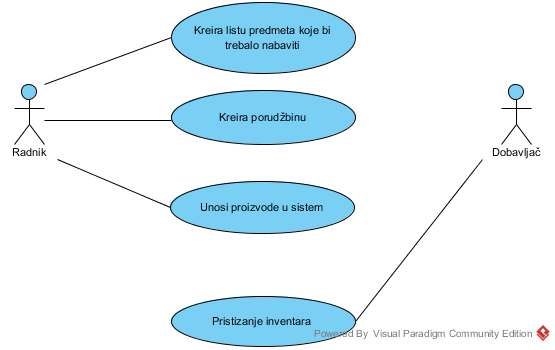
\includegraphics[width=\textwidth]{pregled_inventara.png}
\subsection{\textbf{Use Case}: Pregled stanja inventara}
\textbf{Akter:} Zaposleni restorana\\
\textbf{Ulaz:} Nema\\
\textbf{Izlaz:} 
\begin{enumerate}
	\item Spisak predmeta koji spadaju u inventar ugostiteljskog objekta i njihove zalihe su usled kvara ili nestanka ispod minimalnih definisanih količina.
	\item Lista svih predmeta i njihova trenutna količina.
\end{enumerate} 
\textbf{Preduslovi:} Radnik se uspešno ulogovao na sistem.\\
\textbf{Postuslov:} Uspešno je kreiran spisak predmeta. Ukoliko neki predmet zahteva popravku, lista sadrži tu informaciju.\\
\textbf{Glavni tok:} 
\begin{enumerate}
	\item Radnik se prijavljuje na sistem.
	\item Zahteva od  od sistema spisak predmeta za koje važi da je trenutna količina manja od minimalne propisane ili je neki od aparata u kvaru.
	\item Sistem kreira listu predmeta koji ispunjavaju prethodni zahtev.
\end{enumerate}
\textbf{Alternativni tok:} Ne postoje podaci o minimalnim količinama ni za jedan predmet u sistemu, pa nije moguće kreirati pregled stanja.\\

\subsection{\textbf{Use Case}: Kreiranje porudžbine}
\textbf{Akter:} Zaposleni restorana\\
\textbf{Ulaz:} Lista predmeta čije su zalihe ispod minimalnih definisanih za poslovanje ugostiteljskog objekta.\\
\textbf{Izlaz:} Lista poručenih predmeta.\\
\textbf{Preduslovi:} Radnik ima uvid u spisak predmeta čija je količina manja od poželjne.\\
\textbf{Postuslov:} Porudžbina je kreirana.\\
\textbf{Glavni tok:} 
\begin{enumerate}
	\item Radnik uzima listu predmeta koje bi trebalo nabaviti.
	\item Radnik procenjuje količinu za nabavku. 
	\item Radnik proverava da li postoje predmeti koje želi da uvrsti u inventar i doda ih u porudžbinu.
	\item Kreira porudžbinu.
\end{enumerate}
\textbf{Alternativni tok:} Ukoliko je lista predmeta na minimalnim zalihama prazna, procena količina se ne vrši.\\

\subsection{\textbf{Use Case}:  Pristizanje predmeta i aparata}
\textbf{Akter:} Dobavljač\\
\textbf{Ulaz:} Lista poručenih predmeta.\\
\textbf{Izlaz:} Lista predmeta koje je dobavljač isporučio ugostiteljskom objektu.\\
\textbf{Preduslovi:} Dobavljač je dobio porudžbinu.\\
\textbf{Postuslov:} Predmeti su isporučeni kupcu i kreirana je lista dostavljenih proizvoda.\\
\textbf{Glavni tok:} 
\begin{enumerate}
	\item Dobavljač je dobio listu poručenih proizvoda.
	\item Proverava za svaki proizvod da li je njegova firma u mogućnosti da isporuči tražene količine.
	\item Po potrebi, smanjuje količine koje su poručene.
	\item Isporučuje robu ugostiteljskom objektu.
	\item Pri isporuci dostavljena je lista predmeta koji su isporučeni.
\end{enumerate}
\textbf{Alternativni tok:} Zbog manjka raspoloživih predmeta, dobavljač otkazuje porudžbinu.\\

\subsection{\textbf{Use Case}: Unos predmeta u sistem}
\textbf{Akter:} Radnik\\
\textbf{Ulaz:} Spisak predmeta koje je dobavljač isporučio.\\
\textbf{Izlaz:} Ažurirana je lista predmeta koji čine inventar.\\
\textbf{Preduslovi:} Radnik se uspešno ulogovao na sistem. Dobavljač je dostavio poručene proizvode.\\
\textbf{Postuslov:} Ažurirane su količine proizvoda i eventualno uneti novi.\\
\textbf{Glavni tok:} 

\begin{enumerate}
	\item Radnik je dobio listu isporučenih proizvoda.
	\item Radnik se prijavljuje na sistem.
	\item Za svaki od proizvoda sa liste, radnik ažurira proizvod u sistemu tako što dodaje pristiglu količinu.
	\item Ukoliko proizvod ne postoji u sistemu, radnik kreira proizvod sa njegovim karakteristikama.
	\item Ažurira novokreirani proizvod pristiglom količinom i eventualno definiše minimalnu količinu. 
\end{enumerate}
\textbf{Alternativni tok:} Porudžbina je otkazana, nema unosa.\\


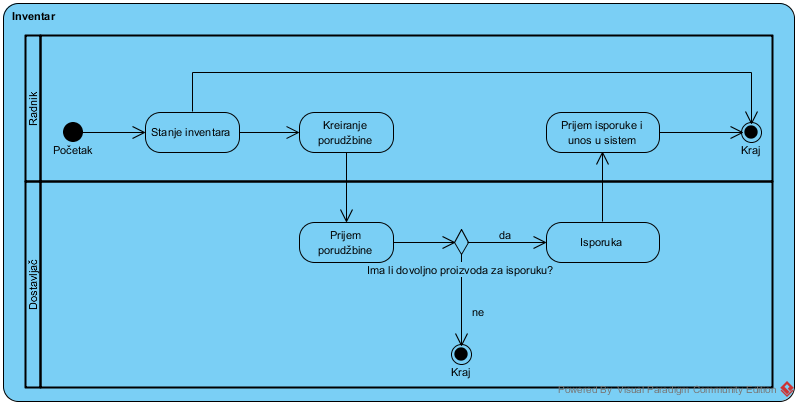
\includegraphics[width=\textwidth]{pregled_inventara_activity.png}
\end{document}
